\begin{figure}
  \centering
  \updatedFigure{
  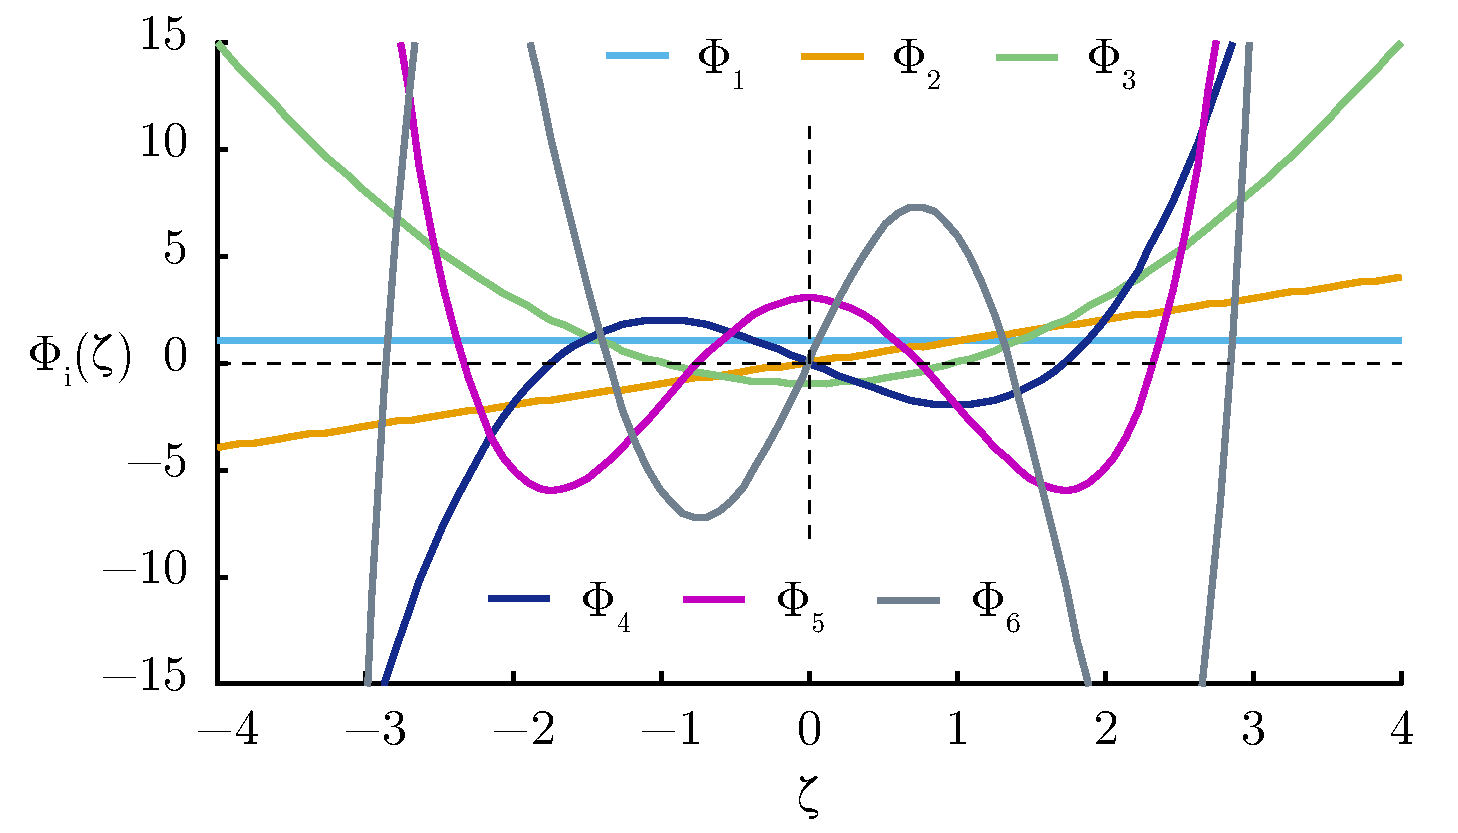
\includegraphics[width=0.9\columnwidth]{include/assets/hermite.pdf}
  }
  \vspace{-1.0em}
  \caption{The first six polynomials of the Hermite basis.}
  \vspace{-1.5em}
  \flabel{hermite}
\end{figure}

The construction of PC expansions is based on the Hermite polynomial basis (see \tref{askey}) as it was found to be optimal in many situations involving Gaussian parameters \cite{xiu2002}. To illustrate the basis, in the one-dimensional setting, the first six Hermite polynomials $\{ \pcb_i(\z) \}_{i = 1}^6$ are those depicted in \fref{hermite}.

Once the basis has been chosen, we need to compute the corresponding coefficients, specifically, $\pcc{\vP}_i$ in \eref{pc-expansion}. As shown in \aref{polynomial-chaos}, $\pcc{\vP}_i$ involve multidimensional integration with respect to the \pdf\ of the \rvs\ $\vZ(\o)$. In numerical analysis, this task is typically accomplished by virtue of a quadrature rule \cite{press2007}, which, loosely speaking, is a weighted summation over the integrand values computed at prescribed points. A natural choice of a quadrature rule when the weight function is a Gaussian \pdf\ is the Gauss-Hermite quadrature. For the clarity of presentation, a detailed explanation of the computational procedure is left to the appendix, \aref{gauss-quadrature}, where an introduction to numerical integration and, in particular, to Gauss quadratures is given.

Up to this point, we have completed four out of five steps of the proposed UQ framework depicted in \fref{algorithm}. The result is a light surrogate model of the problem in \eref{fourier-system}. At each moment of time, the surrogate is essentially two $\cores$-valued polynomials, one for power and one for temperature, which are defined in terms of $\vars$ mutually independend \rvs; an example of such a polynomial is given in \eref{pc-k}. Now, the constructed surrogate can be trivially analyzed to retrieve the needed statistics about the stochastic system in \eref{fourier-system}, and this is the fifth step in \fref{algorithm}, which we shall discuss in the following section.
